% Created 2021-04-21 Wed 11:45
% Intended LaTeX compiler: pdflatex
\documentclass[11pt]{article}
\usepackage[utf8]{inputenc}
\usepackage[T1]{fontenc}
\usepackage{graphicx}
\usepackage{grffile}
\usepackage{longtable}
\usepackage{wrapfig}
\usepackage{rotating}
\usepackage[normalem]{ulem}
\usepackage{amsmath}
\usepackage{textcomp}
\usepackage{amssymb}
\usepackage{capt-of}
\usepackage{hyperref}
\usepackage{caption}
\usepackage{subcaption}
\author{Laurent Lejeune}
\date{\today}
\title{Mojo Fertility Assignment}
\hypersetup{
 pdfauthor={Laurent Lejeune},
 pdftitle={Mojo Fertility Assignment},
 pdfkeywords={},
 pdfsubject={},
 pdfcreator={Emacs 26.3 (Org mode 9.4)}, 
 pdflang={English}}
\begin{document}

\maketitle


\section{Context and Goal}
\label{sec:org857aacc}

In the context of sperm quality assessment, we devise an algorithm that counts the number of spermatozoa
on image-slices obtained through a camera.


\section{Method}
\label{sec:org6c0b983}

Our solution relies on a Random Forest classifier.
In a nutshell, we first leverage the \href{https://www.epfl.ch/labs/cvlab/software/descriptors-and-keypoints/daisy/}{DAISY} descriptors to characterize local regions.
We then devise a sampling strategy to augment the scarce positive set, while a hard negative mining strategy allows to select relevant samples from the redundant and ambiguous
negative set.

The main challenges of this problem lies in (1) the strong imbalance of the provided annotated dataset, where the mean number of positive samples per image is around \(10\), and (2) the fact that many spermatozoa that are not
in focus must be classified as negative.

It is therefore clear that training an efficient classifier in this context requires an appropriate
negative mining strategy, since a vast amount of potential negative samples carry no relevant information, e.g.
homogeneous taint, or obvious artifacts (debris), while many negative samples (out of focus) are visually similar to
positives.

We now describe in more details our pipeline.
After introducing some notations, we describe our feature extraction instance, follow with
our negative mining strategy, and finish by giving details on the setting of hyper-parameters using K-fold cross-validation.


\subsection{Notations}
\label{sec:org333e2f1}

\begin{itemize}
\item \(\bm{X} \in \mathbb{R}^{N \times D}\) a feature matrix where rows are samples and columns
are the components of the feature vector.
\item \(\bm{Y} \in \{0;1\}^N\) the ground-truth label vector of the corresponding samples
\item \(\hat{y}= f_{\theta}(x): \mathbb{R}^{D} \rightarrow [0;1]\) is a classifier that outputs the probability of an input vector to be an object of interest.
\end{itemize}

\subsection{Feature extraction}
\label{sec:org2d4ab11}

DAISY descriptors have been proposed as an improvement over the popular \href{https://en.wikipedia.org/wiki/Scale-invariant\_feature\_transform}{Scale Invariant Feature Transform (SIFT)}.
In particular, it is devised to compute dense descriptors (one per pixel) using a fast algorithm.

In our scenario, we do not need to localize samples precisely.
We therefore prefer to extract descriptors with a decimation step of \(16\) pixels, so as to save memory.
For an image of size \(1920 \times 1200\), we obtain a total of \(9000\) descriptors encoded in \href{https://en.wikipedia.org/wiki/Half-precision\_floating-point\_format}{Half-precision floating-point format}.

The \href{https://github.com/scikit-image/scikit-image/blob/main/skimage/feature/\_daisy.py\#L9-L222}{algorithm} computes dense descriptors in \(\sim 5\) seconds per image, making \(\sim 50\) minutes for the full dataset (500 images).

\subsection{Classifier}
\label{sec:org05b6904}

To classify samples, we use a \href{https://en.wikipedia.org/wiki/Random\_forest}{Random Forest} classifier.
As purity criterion, we select the \href{https://en.wikipedia.org/wiki/Gini\_coefficient}{Gini} index.

\subsection{Augmentation of positives}
\label{sec:org3d60135}

To alleviate the lack of positives, we define a circular region centered on a \((x,y)\) location
annotated as positive, and
take as positive samples all samples whose center is in a close vicinity.
In particular, we compute a pairwise distance matrix between all positives and all other samples,
threshold the values of this matrix by a pre-defined constant \(L_2\) -norm,
and augment our positive set with the corresponding samples.

\subsection{Hard negative mining}
\label{sec:org8abbdc6}

We follow a simple iterative strategy to identify ``hard'' negatives.
As we want our negatives to be \emph{far enough} from positives, we first filter-out negative candidates that are
close to a positive sample by thresholding the \(L_2\) -norm.

Our idea is then to pick relevant negative samples by using the predicted probability of the model itself.

Let \(\mathcal{S}_p\) the set of positive samples, obtained as in Sec. \ref{sec:org3d60135}, such that \(|\mathcal{S}_p|=N_p\).
Also, let \(\mathcal{S}_n\) the set of negative samples, such that \(|\mathcal{S}_n|=N_n \gg N_p\).


We train a Random Forest classifier \(f_\theta\) using the following procedure:

\begin{enumerate}
\item Train \(f_\theta\) by fitting \(T\) trees using positive set \(\mathcal{S}_p\), and negative set \(\mathcal{S}'_n\) with \(N_p\)
samples chosen by uniform random sampling from \(\mathcal{S}_n\).
\item Set \(\mathcal{S}_n \leftarrow \mathcal{S}_n \textbackslash \mathcal{S}'_n\)
\item Predict probabilities of samples in \(\mathcal{S}_n\) using \(f_\theta\) to get \(\hat{y}^-\)
\item Sort \(\mathcal{S}_n\) according to \(\hat{y}^-\), and populate
\(\mathcal{S}'_n\) with the last \(N_p\) elements of \(\mathcal{S}_n\).
\item re-train \(f_\theta\) by fitting \(T\) \textbf{additional} trees using \(\mathcal{S}_p\) and \(\mathcal{S}'_n\).
\item Repeat steps 2-5 \(M\) times.

Fig. \ref{fig:org987e887} illustrates our sampling strategy on an example image.

\begin{figure}[htbp]
\centering
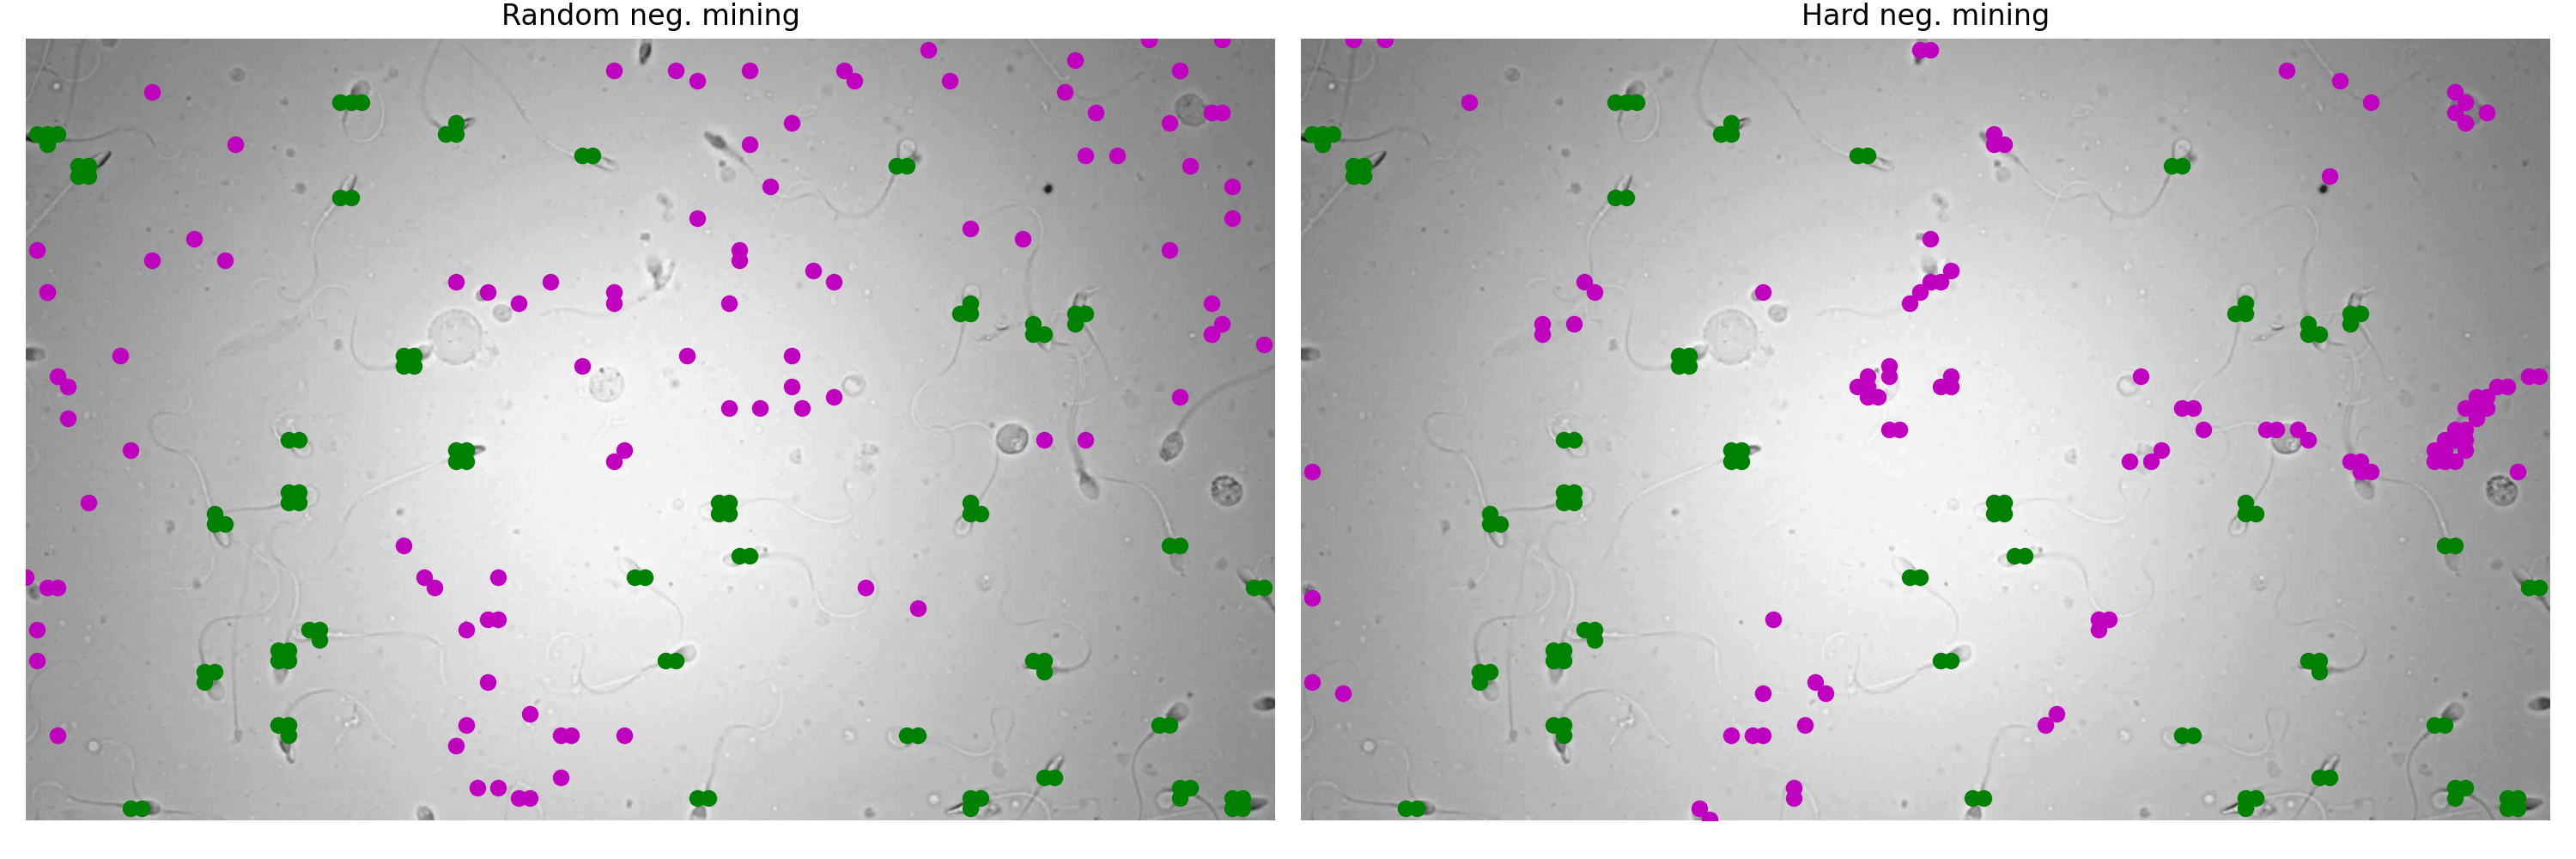
\includegraphics[width=.9\linewidth]{./mining_prev.png}
\caption{\label{fig:org987e887}Sample mining strategy on an image. Positives are in green, negatives are in magenta. Left: For the first iteration, negatives are sampled at random. Right: Negatives are sampled according to our hard mining strategy.}
\end{figure}
\end{enumerate}

\subsection{Post-processing}
\label{sec:org3bafff4}

As a post-processing step, we first apply a threshold \(\tau\) to the probability values given
by our classifier,
and apply a simple non-maximum suppression algorithm to select
in a given spatial neighborhood
the most-likely positive candidate.

\subsection{Tuning of hyper-parameters}
\label{sec:org41e4d75}

We optimize the following hyper-parameters of our classifier using grid-search and 4-fold cross-validation:

\begin{itemize}
\item Maximum number of feature components to pick at each split.
\item Threshold value \(\tau\) applied to the output probabilities.
\end{itemize}

\section{Experiments}
\label{sec:org1ff7864}

So as to demonstrate the relevance of our hard mining strategy, we perform an ablation study.
In particular, we introduce methods:

\begin{itemize}
\item \textbf{Hard Negative Mining Random Forest}: A Random Forest classifiers containing \(M \cdot T\) trees
optimized using an augmented positive set (Sec. \ref{sec:org3d60135} ), and the proposed hard negative mining strategy (Sec. \ref{sec:org8abbdc6}).
\item \textbf{Random Negative Mining Random Forest}: A Random Forest classifiers containing \(M \cdot T\) trees
optimized using the same augmented positive set, and randomly sampled negatives.
\end{itemize}

Both methods are cross-validated (as in Sec. \ref{sec:org41e4d75}) using the same training and validation subsets to get their respective
optimal hyper-parameters.

Using these, we then re-train both methods on an identical data subset (union of training and validation set used in Sec. \ref{sec:org41e4d75}), and compute performance metrics on the remaining set (test set).

Letting \(C_i\) and \(\hat{C}_i\) the true and estimated counts of frame \(i\), respectively, we report as metric the mean absolute normalized count error given by

\[
m = \mathbb{E}_i \left[ \frac{|\hat{C}_i - C_i|}{C_i} \right]
\]

We show our results on Tab. \ref{tab:org51ae428}, and some qualitative results on Fig. \ref{fig:test_prevs}.

\begin{table}[htbp]
\centering
\begin{tabular}{lrr}
Method & m-score & MAE\\
\hline
\textbf{Hard Negative Mining} & 0.49 & 9.01\\
\textbf{Random Negative Mining} & 1.87 & 11.36\\
\end{tabular}
\caption{\label{tab:org51ae428}Performance of proposed methods. We report the mean absolute error (MAE) between the true count and the predicted count, and the mean normalized absolute error (m-score)}

\end{table}


\begin{figure}
     \centering
     \begin{subfigure}[b]{0.4\textwidth}
         \centering
         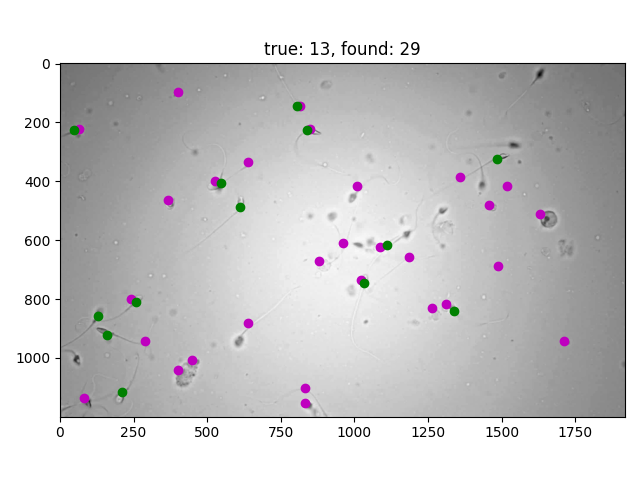
\includegraphics[width=\textwidth]{rnd_result_prev.png}
     \end{subfigure}
     \hfill
     \begin{subfigure}[b]{0.4\textwidth}
         \centering
         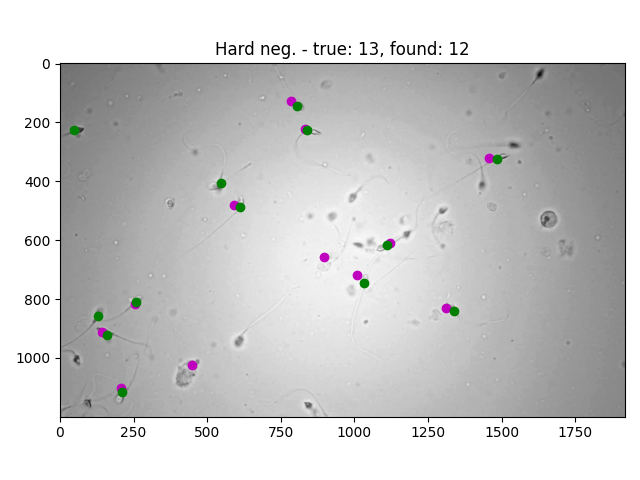
\includegraphics[width=\textwidth]{hard_result_prev.png}
     \end{subfigure}
        \caption{Example of predictions. Groundtruth positives are in green, predicted positives are in magenta
(Left) Random Negative Mining, (Right) Hard Negative Mining.}
        \label{fig:test_prevs}
\end{figure}

\section{Discussion and Conclusion}
\label{sec:orgaa7fc36}

The proposed hard negative mining strategy brings a substantial improvement over the simpler random negative mining.
In particular, we show an improvement of \(74\%\) according to the mean normalized absolute count error.

\subsection{Limitations and potential improvements}
\label{sec:org618ed82}

Given the limited amount of time allocated, as well as limited computational ressources (only CPU-based solutions were considered for practical reasons) to this effort, we suggest the following potential future improvements:

\begin{itemize}
\item A deep learning model could be optimized so as to classify. In particular, the latter approach allows
to optimize both the feature extraction instance and the classification instance in an end-to-end manner.
\item For the present scenario, an even simpler approach could consist in taking the whole image as input,
so as to optimize a regression layer that counts the number of occurrences.

The more complex problem of assessing the motility requires that positive samples are explicitly localized so as to be tracked.
The latter task could be tackled using a region-proposal algorithm.
Litterature already provides efficient solutions, such as \href{https://arxiv.org/abs/1506.01497}{Faster R-CNN},that rely on a CNN and regression layers so as to provide
objectness probabilities along with the coordinates of corresponding bounding-boxes.
However, the present scenario, in my understanding, does not justify the need for these coordinates, as most objects (spermatozoa)
are of equal size.
\end{itemize}

\subsection{Discussion on dataset and annotation}
\label{sec:org65f4a15}

The annotation task contains a strong subjective factor, in that there is no strong frontier between an
in-focus and out-of-focus spermatozoa.

This aspect could be addressed by giving the same dataset to several annotators, so as to
compute a consensus.

Another approach could consist in changing the annotation protocol so as to obtain a negative set that contains out-of-focus spermatozoa and other confusing
artifacts.

\subsection{Discussion on the detection and tracking pipeline}
\label{sec:org74d4c7f}

In order to assess motility, an accurate object detection instance is crucial, but not sufficient.

The latter instance must be coupled with a tracking module that would connect detections over time.
In particular, I believe that multi-object tracking algorithms would be appropriate,
and recommend \href{https://infoscience.epfl.ch/record/164041?ln=en}{Multiple Object Tracking using K-Shortest Paths Optimization (Berclaz et al, 2011)}.
\end{document}
